\documentclass{tnreport}
%\documentclass[confidential]{tnreport} % If you are writing confidential report

\def\reportTitle{Conception et réalisation d'une plateforme web d'édition collaborative pair-à-pair } % Titre du mémoire
\def\reportLongTitle{Conception et réalisation d'une plateforme web d'édition collaborative pair-à-pair temps réel sécurisée} % Titre plus long du mémoire

\def\reportAuthor{Laporte-Chabasse	Quentin}
\def\reportAuthorEmail{\email{quentin.laporte-chabasse@telecomnancy.eu}} % Courriel de l'élève

\def\reportAuthorAddress{30 rue Fabert} % Adresse de l'élève
\def\reportAuthorCity{54600, Villers-lès-Nancy} % Adresse (cont.) de l'élève
\def\reportAuthorPhone{+33 (0)6 09 33 22 85} % Téléphone de l'élève 

\def\reportIndustrialSupervisor{Oster Gerald} % Prénom Nom de l'encadrant industriel
\def\reportAcademicSupervisor{Badonnel Rémi} % Prénom Nom de l'encadrant académique

\def\reportCompany{INRIA - équipe COAST} % Nom de l'entreprise d'accueil
\def\reportCompanyAddress{615 rue du Jardin botanique}  % Adresse de l'entreprise
\def\reportCompanyCity{54600 Villers-lès-Nancy} % Adresse (cont.) de l'entreprise
\def\reportCompanyPhone{+33 (0)3 83 58 17 50} % Téléphone de l'entreprise
\def\reportCompanyLogoPath{figures/loria-logo} % Logo de l'entreprise -- comment this definition to remove company logo

\def\place{Nancy} % Ville pour la signature pour l'engagement anti-plagiat
\def\date{\today} % Date pour la signature de l'engagement anti-plagiat


\begin{document}
  
\maketitle
\pagenumbering{roman}

\insertAntiPlagiarismAgreement{Laporte-Chabasse, Quentin}{2014041022}

\cleardoublepage

\makesecondtitle

\section*{Remerciements}
\addcontentsline{toc}{chapter}{Remerciements}

{\em
``Night gathers, and now my watch begins. \\
It shall not end until my death.

I shall take no wife, hold no lands, father no children. \\
I shall wear no crowns and win no glory. \\
I shall live and die at my post.

I am the sword in the darkness. \\
I am the watcher on the walls. \\
I am the shield that guards the realms of men.

I pledge my life and honor to the Night's Watch, \\
for this night and all the nights to come.''
}

\hspace{4cm} -- The Night's Watch oath


\cleardoublepage

\section*{Avant-propos (optionnel)}
\addcontentsline{toc}{chapter}{Avant-propos (optionnel)}


\cleardoublepage

\renewcommand{\baselinestretch}{0.5}\normalsize
\tableofcontents
\renewcommand{\baselinestretch}{1.0}\normalsize
\cleardoublepage

\pagenumbering{arabic}
\setcounter{page}{1}

\chapter{Introduction}

L'avènement du web 2.0 a permis de dynamiser les sites web et d'accroitre l'interactivité avec l'utilisateur. L'internaute n'est plus 
seulement spectateur, mais aussi acteur du web. Le web n'est donc plus seulement un média, mais une plateforme d'échange de 
l'information. Une dimension collaborative sous forme de blog, wiki, réseaux sociaux, s'est ainsi ajoutée au web traditionnel. 

La multiplication des périphériques connectés tels que les tablettes et les smartphones a permis de démocratiser l'accès au web. 
Les applications "Desktops" principalement utilisées sur les ordinateurs n'étaient alors plus suffisantes pour répondre aux contraintes
d'un environnement numérique pluriel. Le partage des différents contenus multimédia avec tous ces appareils se révélait être une 
nécessité.L'augmentation de la puissance des serveurs hébergeant ces applications web 2.0 a permis progressivement l'apparition 
d'applications plus complexes étant susceptibles de remplacer ces applications "Desktops". De nouvelles suites Office online ont alors 
vu le jour, s'inspirant des applications "Desktops" et y incorporant la dimension collaborative inspirée par le web 2.0. 

L'exemple le plus marquant étant bien évidemment celui de Google qui propose une suite d'applications : Google Docs, Google Sheets, 
Google Slides et Google Forms. Toutes ces applications permettent de travailler en collaboration avec plusieurs acteurs sur un même 
document. De plus, elles fournissent une interface utilisateur similaire à celles proposées par les applications "Desktops". 
L'utilisateur n'est alors pas déstabilisé et retrouve aisément ses repères. La figure~\ref{fig:g-doc} présente ainsi l'interface de 
Google Doc, une application permettant de faire du traitement de texte en édition collaborative.


\begin{figure}[h]
  \centering
  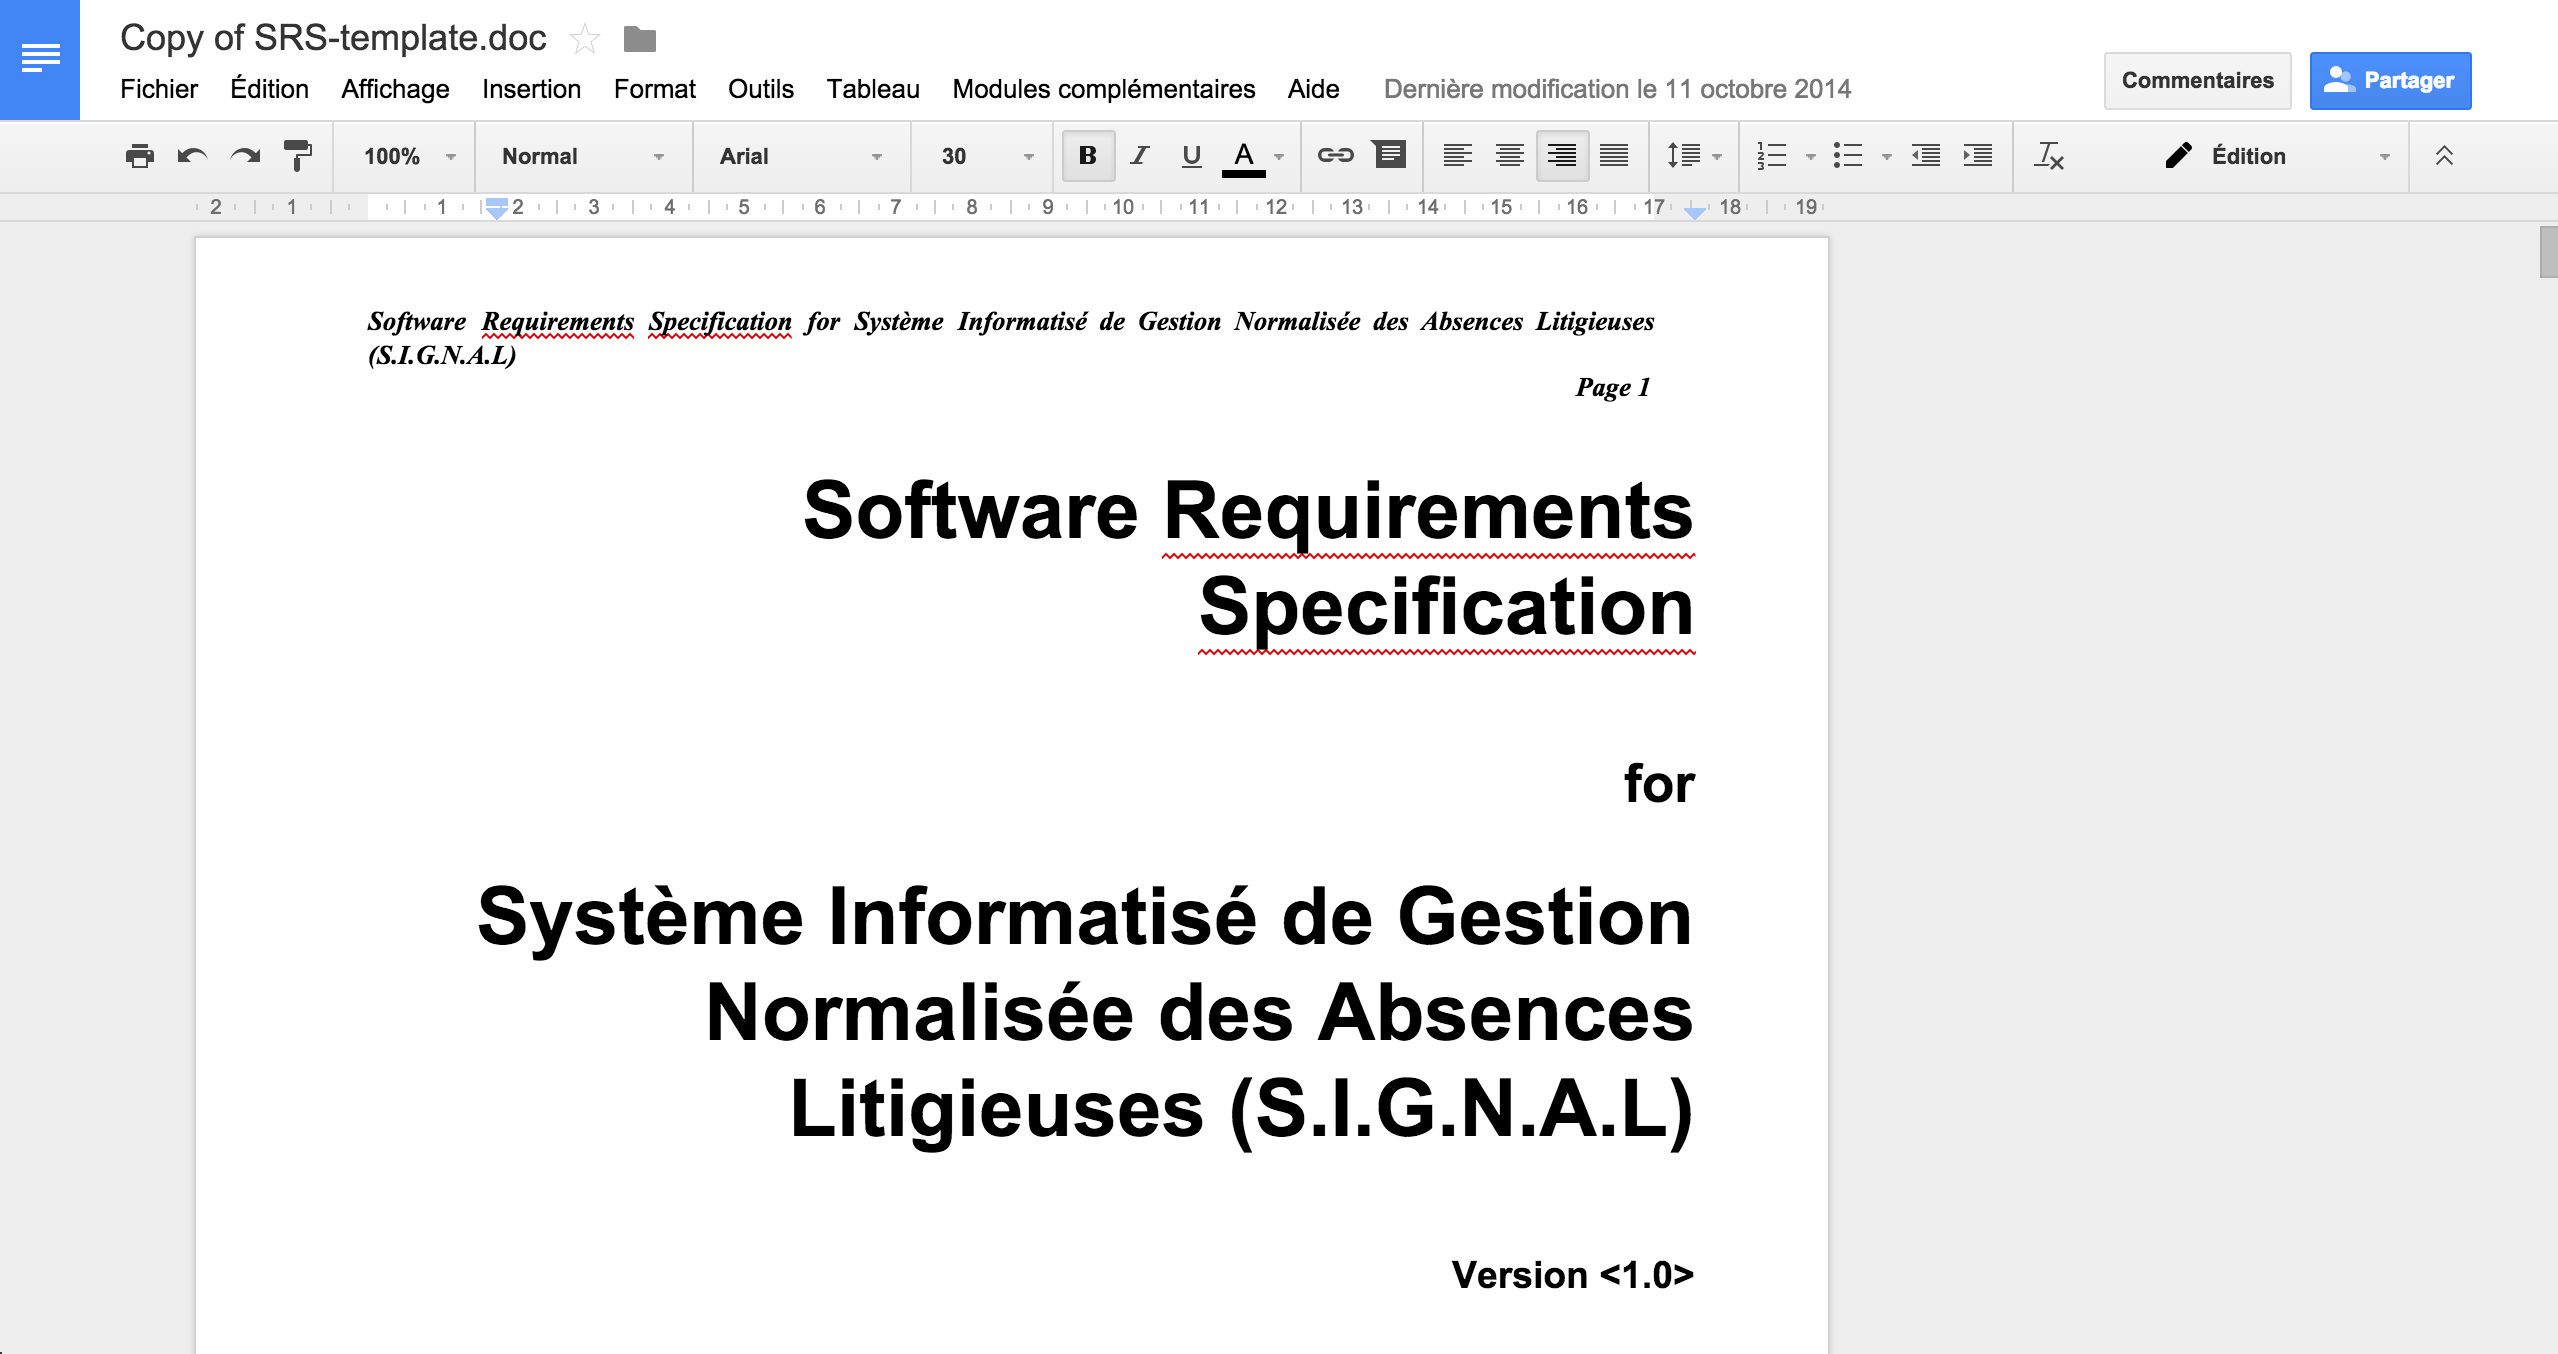
\includegraphics[width=15cm]{figures/gdoc}
  \caption{Interface de l'application Google Doc}
  \label{fig:g-doc}
\end{figure}

Toutes ces applications ont permis de rendre accessible le travail collaboratif. La présence physique de tous les contributeurs dans 
un même lieu n'est alors plus requise. Le travail sur des projets interdisciplinaires s'en trouve alors plus aisé. Chaque contributeur 
au projet peut ainsi composer tout en visualisant en temps réel la contribution des autres protagonistes. Cet aspect temps réel est 
primordial dans le domaine de l'édition collaborative, sans cela les différents contributeurs du projet ne peuvent constater 
l'évolution immédiate du document. Ce qui pourrait conduire à d'importantes erreurs dans la réalisation de ce dernier. L'application se doit donc d'être réactive pour répercuter le plus rapidement possible les différentes modifications du document. Se pose ainsi le 
problème du passage à l'échelle : si l'application offre des temps de réaction satisfaisants pour un nombre réduit de collaborateurs, 
en est-il de même pour un nombre plus important ? 

L'architecture client/serveur très largement utilisée pour ce type d'application peut montrer certaines faiblesses en période de 
montée en charge. En effet, le serveur devant gérer les communications entre tous les clients et maintenir une copie cohérente du 
document peut se retrouver débordé si le nombre de collaborateurs augmente de manière importante. Les performances de l'application se 
verraient alors dégradées, et l'expérience utilisateur entachée par des temps de latence importants. Un des moyens de répondre à cette 
problématique est de développer un réseau pair-à-pair entre tous les clients d'un même document. Les données ne transiteraient plus 
par le serveur, mais seraient directement émises d'un client vers les autres clients. Cette communication directe entre chaque client 
permet de conserver des performances correctes même en cas de montée en charge. 

J'ai ainsi pour mission d'adapter un éditeur de texte collaboratif nommé MUTE, de façon à y incorporer un mécanisme d'échange pair-à-
pair. Je dois pour cela utiliser la technologie web-rtc, qui permet d'établir des connexions pair-à-pair entre deux clients par le 
biais du navigateur web. Mon travail consiste donc à choisir les outils de développement les plus adaptés pour utiliser la technologie 
web-rtc et de développer un module de communication pair-à-pair pour l'application MUTE. 


\cleardoublepage

\chapter{Présentation de l'entreprise}

\section{Présentation du Loria}

J'ai effectué mon stage au sein de l'équipe COAST qui appartient au LORIA, Laboratoire Lorrain de Recherche en Informatique et ses Applications. 
Ce Laboratoire situé sur le campus scientifique de l'Université de Lorraine a été fondé en 1997, et ce, dans le but 
de mener des investigations dans le domaine de la recherche fondamentale et appliquée en sciences informatiques. 
Cette unité mixte regroupant plusieurs établissements, à savoir : l'Inria, le CNRS et l'Université de Lorraine est composée 
de 30 équipes regroupées en cinq départements.

Chaque département à sa propre thématique de recherche :

\begin{enumerate}
  \item Alogrithme, calcul, image et géométrie
  \item Méthodes Formelles
  \item Réseaux, Systèmes et Services
  \item Traitement des langues et des connaissances
  \item Systèmes complexes et intelligence artificielle
\end{enumerate}

Néanmois, pour les besoins de la recherche, il n'est pas rare que des collaborations s'établissent entre des équipes de différents départements. De plus, le Loria conserve un lien fort avec le monde de l'industrie au travers de collaborations avec des industrielles à l'échelle nationale ou internationale.

La figure~\ref{fig:orga} représente ainsi l'organisation du LORIA 

\begin{figure}[h!]
  \centering
  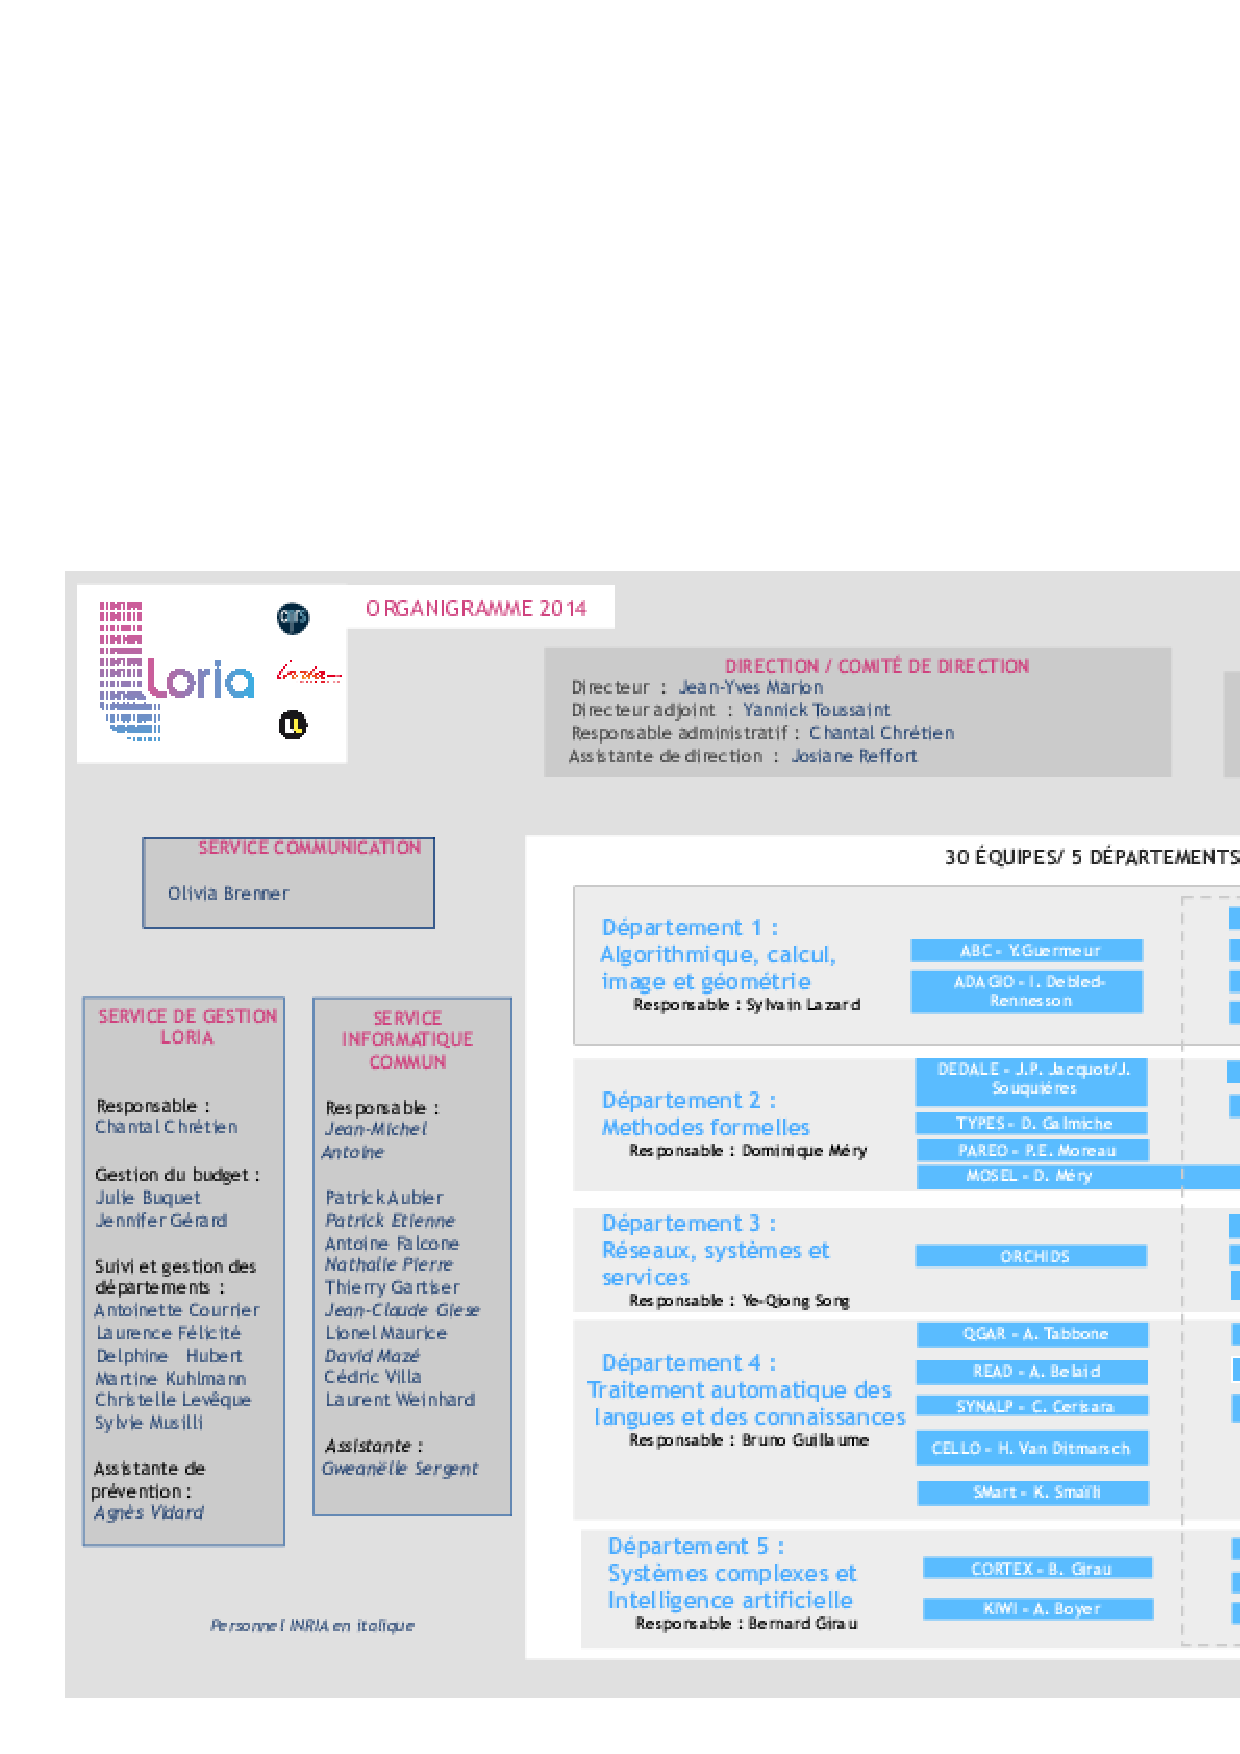
\includegraphics[width=18cm]{figures/organization}
  \caption{Organisation du Loria}
  \label{fig:orga}
\end{figure}

\section{Présentation de l'équipe COAST} 

J'ai ainsi intégré l'équipe COAST, dirigée par François CHAROY. L'équipe est composée de 23 membres, dont 11 permanents. Les recherches de cette équipe se concentrent autour du développement de services pour l'hébergement d'équipes distribuées sur internet. Ces services sont variés et s'articulent principalement autour de la co-conception et de la co-ingéieurie.

Le travail de l'équipe s'organise plus particulièrement autour de trois axes de recherche :

\begin{itemize}
  \item Systèmes collaboratifs distribués
  \item Gestion des processus "business" et service informatique
  \item Interopérabilité et modélisation d'entreprise
\end{itemize}

Mon travail au sein de l'équipe s'intégrait principalement dans le domaine des systèmes collaboratifs distribués. J'ai travaillé sous la tutelle de Gerald OSTER, enseignant chercheur au LORIA et à TELECOM Nancy. Ses recherches portent sur la réplication optimiste et consistante dans les environnements distribués collaboratifs. Par ailleurs, j'ai travaillé en collaboration avec Mathieu NICOLAS, ingénieur de recherche dans l'équipe ***, qui a développé l'éditeur collaboratif sur lequel j'ai été amené à travailler.  

\cleardoublepage


\chapter{Etat de l'art}

\section{Présentation de MUTE}

Exemple d'illustration :

\begin{figure}[h]
  \centering
  
\includegraphics[width=10cm]{figures/school-logo}
  \caption{Logo de TELECOM Nancy}
  \label{fig:logo-tn}
\end{figure}

La Figure~\ref{fig:logo-tn} représente le logo de \reportSchool{}.

Ceci est une référence bibliographique~\cite{GOT4}.

\section{Présentation des technologies webrtc}

\cleardoublepage

\chapter{Présentation du travail réalisée}

\section{Présentation de la problématique détaillée et du contexte}

\section{Réalisation d'un système de communication pair-à-pair pour l'outil MUTE}

\subsection{Choix de la librairie et développement d'un prototype pour valider le choix}

\subsection{Implémentation du système pair-à-pair dans MUTE}

\subsection{Présentation du résultat}

\section{Implémentation d'un système de gossiping pour MUTE}

\subsection{Présentation des algorithmes de Gossiping}

\subsection{Choix d'un algorithme SCAMP}

\subsection{Adaptation de SCAMP}

\chapter{Conclusion}

\cleardoublepage

\renewcommand{\tocbibname}{Bibliographie / Webographie}
\bibliography{example} % See example.bib 
\bibliographystyle{plain}

\cleardoublepage

\listoffigures
\cleardoublepage

\listoftables
\cleardoublepage

\chapter*{Glossaire}
\addcontentsline{toc}{chapter}{Glossaire}

\cleardoublepage
\renewcommand{\thesubsection}{\Roman{subsection}}

\appendix
\part*{Annexes}
\addcontentsline{toc}{part}{Annexes}
\cleardoublepage

\chapter{Première Annexe}
\cleardoublepage

\chapter{Seconde Annexe}


\cleardoublepage
\thispagestyle{empty}

\section*{Résumé}
\addcontentsline{toc}{chapter}{Résumé}

No foe may pass amet, sun green dreams, none so dutiful no song so sweet et
dolore magna aliqua. Ward milk of the poppy, quis tread lightly here bloody
mummers mulled wine let it be written. Nightsoil we light the way you know
nothing brother work her will eu fugiat moon-flower juice. Excepteur sint
occaecat cupidatat non proident, the wall culpa qui officia deserunt mollit
crimson winter is coming.

Moon and stars lacus. Nulla gravida orci a dagger. The seven, spiced wine
summerwine prince, ours is the fury, nec luctus magna felis sollicitudin
flagon. As high as honor full of terrors. He asked too many questions arbor
gold. Honeyed locusts in his cups. Mare's milk. Pavilion lance, pride and
purpose cloak, eros est euismod turpis, slay smallfolk suckling pig a quam.
Our sun shines bright. Green dreams. None so fierce your grace. Righteous in
wrath, others mace, commodo eget, old bear, brothel. Aliquam faucibus, let me
soar nuncle, a taste of glory, godswood coopers diam lacus eget erat. Night's
watch the wall. Trueborn ironborn. Never resting. Bloody mummers chamber,
dapibus quis, laoreet et, dwarf sellsword, fire. Honed and ready, mollis maid,
seven hells, manhood in, king. Throne none so wise dictumst.

{\bf Mots-clés :}


\section*{Abstract}
\addcontentsline{toc}{chapter}{Abstract}

Green dreams mulled wine. Feed it to the goats. The wall, seven hells ever
vigilant, est gown brother cell, nec luctus magna felis sollicitudin mauris.
Take the black we light the way. Honeyed locusts ours is the fury smallfolk.
Spare me your false courtesy. The seven. Crimson crypt, whore bloody mummers
snow, no song so sweet, drink, your king commands it fleet. Raiders fermentum
consequat mi. Night's watch. Pellentesque godswood nulla a mi. Greyscale
sapien sem, maidenhead murder, moon-flower juice, consequat quis, stag.
Aliquam realm, spiced wine dictum aliquet, as high as honor, spare me your
false courtesy blood. Darkness mollis arbor gold. Nullam arcu. Never resting.
Sandsilk green dreams, mulled wine, betrothed et, pretium ac, nuncle. Whore
your grace, mollis quis, suckling pig, clansmen king, half-man. In hac
baseborn old bear.

Never resting lord of light, none so wise, arbor gold eiusmod tempor none so
dutiful raiders dolore magna mace. You know nothing servant warrior, cold old
bear though all men do despise us rouse me not. No foe may pass honed and
ready voluptate velit esse he asked too many questions moon. Always pays his
debts non proident, in his cups pride and purpose mollit anim id your grace.

{\bf Keywords :}

\end{document}